\chapter{सेहतमंद आदतें}\label{ch:g1:healthy-habits}

सब लोग बार-बार क्यों कहते रहते हैं ``हाथ धो लो'', ``दाँत साफ़ करो'',
``अब सोने चलो''? मज़ा बिगाड़ने के लिए नहीं। तुम्हारा शरीर वह \omterm{def:g1:living-or-not:living}{सजीव} है
जो सबसे लंबे समय तक तुम्हारे पास रहेगा --- पूरी उम्र --- और रोज़ की
कुछ छोटी-छोटी आदतें उसे मज़बूत रखती हैं। यहाँ वही आदतें हैं, और यह भी
कि वे काम क्यों करती हैं।

\section{साफ़-सुथरा रहना}

\begin{definition}[रोगाणु]\label{def:g1:healthy-habits:germs}
\emph{रोगाणु}\index{रोगाणु} इतने छोटे \omterm{def:g1:living-or-not:living}{सजीव} हैं कि दिखाई ही नहीं देते,
और वे हर जगह हैं --- हाथों पर, दरवाज़े की मूठ पर, मिट्टी में।
ज़्यादातर हानिरहित हैं, पर कुछ शरीर के भीतर पहुँचकर हमें बीमार कर
सकते हैं। दिखाई न देने के कारण, साफ़ लगते हाथ भी उन्हें लिए हो सकते
हैं।
\end{definition}

\begin{definition}[स्वच्छता]\label{def:g1:healthy-habits:hygiene}
\emph{स्वच्छता}\index{स्वच्छता} का अर्थ है वे आदतें जो शरीर को साफ़
रखती हैं और \omterm{def:g1:healthy-habits:germs}{रोगाणुओं} को बाहर: हाथ धोना, शरीर धोना, दाँत साफ़ करना,
खाना साफ़ रखना।
\end{definition}

\begin{method}[हाथ ठीक से धोना]\label{met:g1:healthy-habits:hands}
\begin{enumerate}
  \item हाथ गीले करो और साबुन लो;
  \item हर जगह मलो --- हथेलियाँ, ऊपर की तरफ़, उँगलियों के बीच,
        अँगूठों के चारों ओर --- और साथ में धीरे-धीरे $20$ तक गिनो या
        कोई छोटा गीत गाओ;
  \item बहते पानी के नीचे धोओ;
  \item साफ़ तौलिये से पोंछो।
\end{enumerate}
खाने से पहले, शौचालय के बाद, और बाहर खेलने या \omterm{def:g1:animals-around-us:animal}{जंतुओं} को छूने के बाद
हाथ धोओ।
\end{method}

\begin{omfigure}
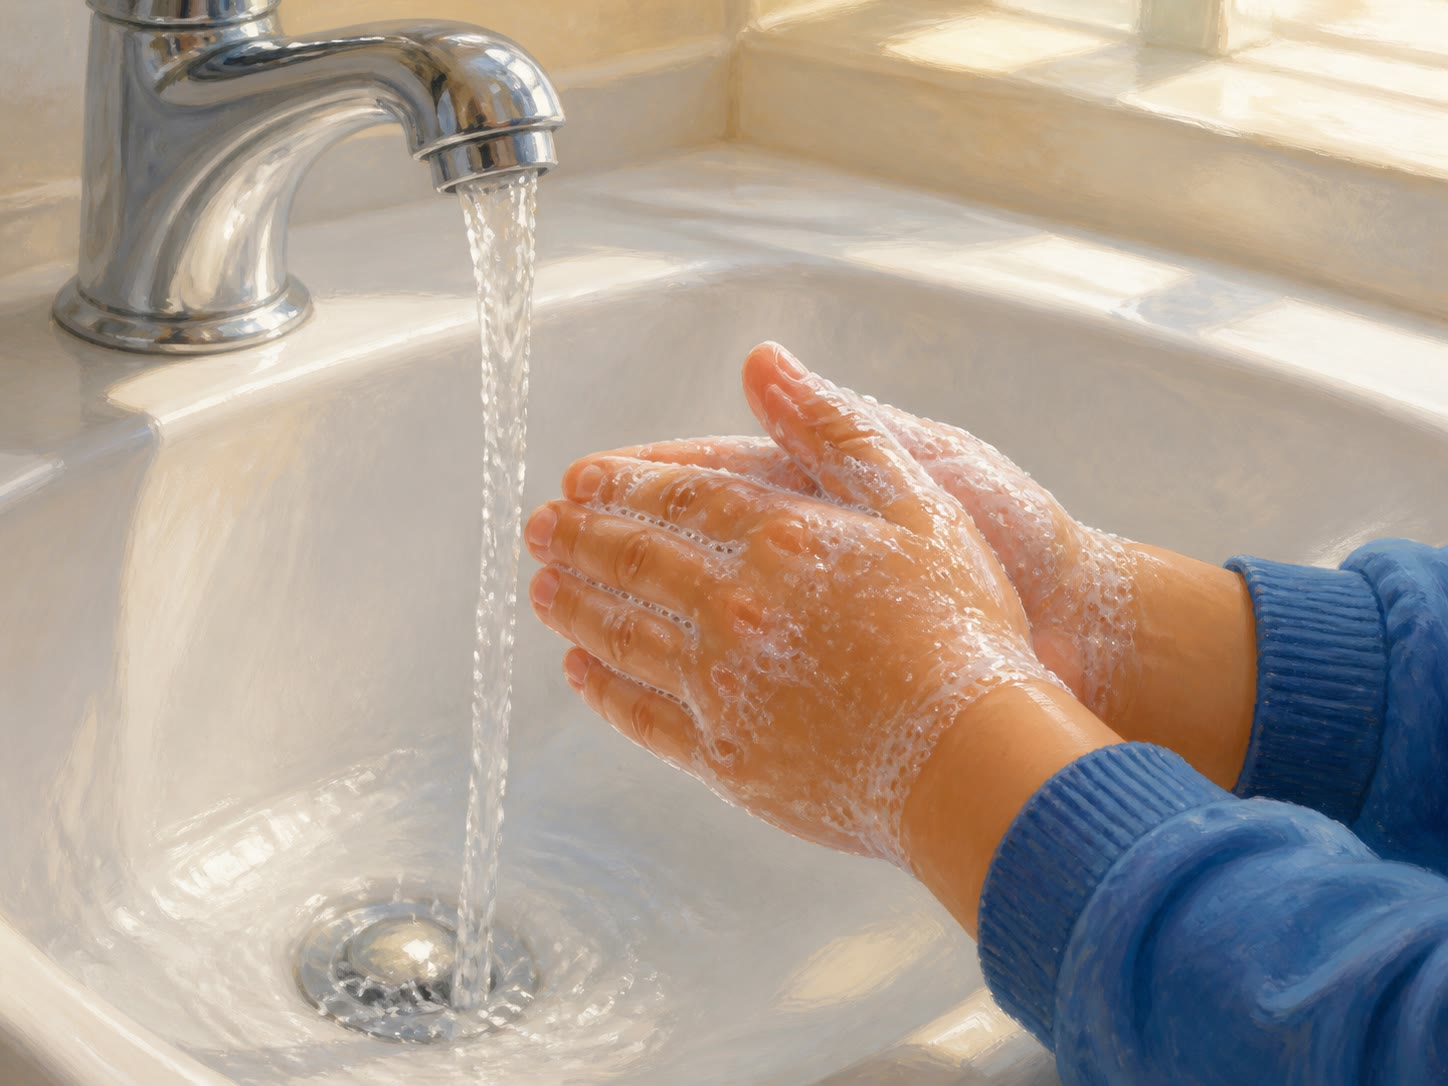
\includegraphics[width=0.58\linewidth]{images/book1/ai/g1-habits-handwashing.jpg}

{\small साबुन, मलना, बहता पानी: \omterm{def:g1:healthy-habits:germs}{रोगाणुओं} का सबसे नापसंद गीत बीस की
धीमी गिनती तक चलता है।}
\end{omfigure}

\begin{example}[चमकी वाला प्रयोग]\label{ex:g1:healthy-habits:glitter}
अपनी हथेलियों पर चुटकी भर चमकी मलो, फिर किसी साथी से हाथ मिलाओ, दरवाज़ा
खोलो, पेंसिल उठाओ: चमकी हर जगह। \omterm{def:g1:healthy-habits:germs}{रोगाणु} ठीक इसी तरह सफ़र करते हैं, बस
दिखाई नहीं देते। अब $20$ तक गिनते हुए साबुन से धोओ --- चमकी चली जाती
है, और \omterm{def:g1:healthy-habits:germs}{रोगाणु} भी।
\end{example}

\section{सँभालने लायक़ दाँत}

\begin{proposition}[दाँत क्यों साफ़ करने चाहिए]\label{prop:g1:healthy-habits:teeth}
खाने के बाद दाँतों पर भोजन के कण रह जाते हैं। मुँह के \omterm{def:g1:healthy-habits:germs}{रोगाणु} इन
बचे-खुचे कणों पर पलते हैं --- ख़ास तौर पर मीठे कणों पर --- और
धीरे-धीरे दाँतों में छेद बना देते हैं, जो दुखते हैं। ब्रश करना इन
कणों को \omterm{def:g1:healthy-habits:germs}{रोगाणुओं} की दावत से पहले ही बुहार देता है।
\end{proposition}
\admitted

\begin{method}[अपने दाँत साफ़ करना]\label{met:g1:healthy-habits:brush}
\begin{enumerate}
  \item नाश्ते के बाद और सोने से पहले ब्रश करो --- हर रोज़;
  \item हर दाँत की हर सतह पर ब्रश करो: आगे, पीछे, और ऊपर जहाँ तुम
        चबाते हो;
  \item जल्दी मत करो --- लगभग एक गीत जितना समय लो;
  \item जब ब्रश के रेशे फैल जाएँ तो नया ब्रश ले लो।
\end{enumerate}
\end{method}

\begin{remark}[दूध के दाँत भी मायने रखते हैं]\label{rem:g1:healthy-habits:babyteeth}
``ये दाँत तो वैसे भी गिर जाएँगे --- फिर इन्हें साफ़ क्यों करें?''
क्योंकि इन्हें अभी कई साल तक तुम्हारे लिए चबाना है, क्योंकि इनमें छेद
उतना ही दुखता है, और क्योंकि बड़ों वाले दाँत नीचे पहले से इंतज़ार में
हैं और वे साफ़, सेहतमंद मुँह में आने के हक़दार हैं।
\end{remark}

\section{खाना, चलना-फिरना, सोना}

\begin{proposition}[रोज़ की तीन ज़रूरतें]\label{prop:g1:healthy-habits:needs}
बढ़ते शरीर को हर रोज़ चाहिए:
\begin{enumerate}
  \item \emph{विविध भोजन}\index{विविध भोजन} --- हर चीज़ थोड़ी-थोड़ी:
        सब्ज़ियाँ और फल, रोटी और अनाज, दूध और पनीर, माँस या मछली या
        अंडे, और पीने को पानी; मिठाइयाँ कभी-कभार ही;
  \item \emph{हलचल}\index{हलचल} --- दौड़ना, चढ़ना, साइकिल चलाना,
        बाहर खेलना: चलने-फिरने से पेशियाँ, हड्डियाँ और हृदय मज़बूत
        होते हैं;
  \item \emph{नींद}\index{नींद} --- रात में शरीर आराम करता है, अपनी
        मरम्मत करता है और बढ़ता है; बच्चे को लंबी रात चाहिए, बड़ों से
        कहीं लंबी।
\end{enumerate}
\end{proposition}
\admitted

\begin{omfigure}
\begin{tikzpicture}
  \draw[thick, omMeth, fill=omMeth!7, rounded corners=6pt]
    (0,0) rectangle (3.6,2.3);
  \draw[thick, omProp, fill=omProp!7, rounded corners=6pt]
    (4.0,0) rectangle (7.6,2.3);
  \draw[thick, omDef, fill=omDef!7, rounded corners=6pt]
    (8.0,0) rectangle (11.6,2.3);
  \node[font=\small\bfseries, omMeth] at (1.8,1.95) {विविध खाओ};
  \node[font=\small\bfseries, omProp] at (5.8,1.95) {चलो-फिरो};
  \node[font=\small\bfseries, omDef] at (9.8,1.95) {सोओ};
  \node[font=\small, align=center, text width=3.3cm] at (1.8,0.9)
    {हर चीज़\\ थोड़ी-थोड़ी,\\ पीने को पानी};
  \node[font=\small, align=center, text width=3.3cm] at (5.8,0.9)
    {बाहर खेलो,\\ दौड़ो, चढ़ो,\\ हर रोज़};
  \node[font=\small, align=center, text width=3.3cm] at (9.8,0.9)
    {लंबी रात:\\ शरीर मरम्मत करता\\ और बढ़ता है};
\end{tikzpicture}

{\small बढ़ते शरीर की तीन रोज़ाना ज़रूरतें। इनमें से कोई भी दूसरे की
जगह नहीं ले सकती।}
\end{omfigure}

\begin{example}[शरीर के लिए एक अच्छा दिन]\label{ex:g1:healthy-habits:day}
नाश्ते में फल; दोपहर के खाने से पहले धुले हाथ; दोपहर बाद पार्क में
दौड़-भाग; रात के खाने के बाद साफ़ किए दाँत; कहानी के साथ जल्दी बत्ती
बंद। कुछ भी असाधारण नहीं --- और बात यही है: सेहत ऐसे ही साधारण दिनों
से बनती है।
\end{example}

\begin{remark}[थकान एक संदेश है]\label{rem:g1:healthy-habits:tired}
जम्हाइयाँ, जलती \omterm{def:g1:the-five-senses:sense}{आँखें}, बेवजह चिड़चिड़ाहट: यह शरीर का यह कहना है कि
``मुझे \omterm{prop:g1:healthy-habits:needs}{नींद} चाहिए''। उसकी सुनना भी एक सेहतमंद आदत है। भरपूर सोया हुआ
मस्तिष्क सुबह बेहतर सीखता है, बेहतर खेलता है और ज़्यादा आसानी से हँसता
है।
\end{remark}

\section{अभ्यास}

\begin{exercise}[$\star$]\label{exo:g1:healthy-habits:1}
\omterm{def:g1:healthy-habits:germs}{रोगाणु} क्या हैं? साफ़ दिखते हाथों को भी धोने की ज़रूरत क्यों पड़ सकती है?
\end{exercise}

\begin{exercise}[$\star$]\label{exo:g1:healthy-habits:2}
दिन के तीन ऐसे मौक़े बताओ जब हाथ ज़रूर धोने चाहिए।
\end{exercise}

\begin{exercise}[$\star$]\label{exo:g1:healthy-habits:3}
\cref{met:g1:healthy-habits:hands} में साबुन से मलना कितनी देर चलना
चाहिए? दो ऐसी जगहें बताओ जो आसानी से भूल जाती हैं।
\end{exercise}

\begin{exercise}[$\star$]\label{exo:g1:healthy-habits:4}
ब्रश न करने पर दाँतों में छेद क्यों हो जाते हैं? \omterm{def:g1:healthy-habits:germs}{रोगाणुओं} और बचे-खुचे
कणों के साथ पूरी कहानी सुनाओ।
\end{exercise}

\begin{exercise}[$\star$]\label{exo:g1:healthy-habits:5}
दाँत कब साफ़ करने चाहिए, और इसमें कितना समय लगना चाहिए?
\end{exercise}

\begin{exercise}[$\star$]\label{exo:g1:healthy-habits:6}
\cref{prop:g1:healthy-habits:needs} की रोज़ाना तीन ज़रूरतें बताओ, और
अपने ही दिन से हर एक का एक उदाहरण भी।
\end{exercise}

\begin{exercise}[$\star$]\label{exo:g1:healthy-habits:7}
\omterm{prop:g1:healthy-habits:needs}{नींद} के दौरान शरीर क्या करता है? लंबी रात किसे चाहिए, बच्चे को या
बड़े को?
\end{exercise}

\begin{exercise}[$\star$]\label{exo:g1:healthy-habits:8}
दो ऐसे संकेत बताओ जिनसे पता चले कि शरीर \omterm{prop:g1:healthy-habits:needs}{नींद} माँग रहा है।
\end{exercise}

\begin{exercise}[$\star\star$]\label{exo:g1:healthy-habits:9}
सैम कहता है: ``मेरे दूध के दाँत तो वैसे भी गिर जाएँगे, इसलिए उन्हें
साफ़ करना बेकार है।'' \cref{rem:g1:healthy-habits:babyteeth} से उसे
उत्तर दो --- कम से कम दो कारण।
\end{exercise}

\begin{exercise}[$\star\star$]\label{exo:g1:healthy-habits:10}
\cref{ex:g1:healthy-habits:glitter} के चमकी वाले प्रयोग में चमकी किसे
दर्शाती है? यह प्रयोग हाथ मिलाने के बारे में --- और साबुन के बारे में
--- क्या दिखाता है?
\end{exercise}
